% Options for packages loaded elsewhere
\PassOptionsToPackage{unicode}{hyperref}
\PassOptionsToPackage{hyphens}{url}
\documentclass[
  american,
  12pt,
  letterpaper,
]{article}
\usepackage{xcolor}
\usepackage{amsmath,amssymb}
\setcounter{secnumdepth}{5}
\usepackage{iftex}
\ifPDFTeX
  \usepackage[T1]{fontenc}
  \usepackage[utf8]{inputenc}
  \usepackage{textcomp} % provide euro and other symbols
\else % if luatex or xetex
  \usepackage{unicode-math} % this also loads fontspec
  \defaultfontfeatures{Scale=MatchLowercase}
  \defaultfontfeatures[\rmfamily]{Ligatures=TeX,Scale=1}
\fi
\usepackage{lmodern}
\ifPDFTeX\else
  % xetex/luatex font selection
\fi
% Use upquote if available, for straight quotes in verbatim environments
\IfFileExists{upquote.sty}{\usepackage{upquote}}{}
\IfFileExists{microtype.sty}{% use microtype if available
  \usepackage[]{microtype}
  \UseMicrotypeSet[protrusion]{basicmath} % disable protrusion for tt fonts
}{}
\makeatletter
\@ifundefined{KOMAClassName}{% if non-KOMA class
  \IfFileExists{parskip.sty}{%
    \usepackage{parskip}
  }{% else
    \setlength{\parindent}{0pt}
    \setlength{\parskip}{6pt plus 2pt minus 1pt}}
}{% if KOMA class
  \KOMAoptions{parskip=half}}
\makeatother
\usepackage{graphicx}
\makeatletter
\newsavebox\pandoc@box
\newcommand*\pandocbounded[1]{% scales image to fit in text height/width
  \sbox\pandoc@box{#1}%
  \Gscale@div\@tempa{\textheight}{\dimexpr\ht\pandoc@box+\dp\pandoc@box\relax}%
  \Gscale@div\@tempb{\linewidth}{\wd\pandoc@box}%
  \ifdim\@tempb\p@<\@tempa\p@\let\@tempa\@tempb\fi% select the smaller of both
  \ifdim\@tempa\p@<\p@\scalebox{\@tempa}{\usebox\pandoc@box}%
  \else\usebox{\pandoc@box}%
  \fi%
}
% Set default figure placement to htbp
\def\fps@figure{htbp}
\makeatother
\ifLuaTeX
\usepackage[bidi=basic,shorthands=off]{babel}
\else
\usepackage[bidi=default,shorthands=off]{babel}
\fi
\ifLuaTeX
  \usepackage{selnolig} % disable illegal ligatures
\fi
\setlength{\emergencystretch}{3em} % prevent overfull lines
\providecommand{\tightlist}{%
  \setlength{\itemsep}{0pt}\setlength{\parskip}{0pt}}
\usepackage[margin=1.24in]{geometry}
\usepackage{setspace}
\usepackage{graphicx}
\usepackage{xcolor}
\usepackage{helvet}
\usepackage{titlesec}
\usepackage{fancyhdr}
\usepackage{booktabs}
\usepackage{longtable}
\usepackage{array}
\usepackage{hyperref}
\definecolor{BookGold}{HTML}{FFD166}
\definecolor{BookBone}{HTML}{F6E8C8}
\definecolor{BookEmber}{HTML}{FF5E3A}
\definecolor{BookInk}{HTML}{12171F}
\renewcommand{\familydefault}{\rmdefault}
\setstretch{1.31}
\setlength{\parindent}{0pt}
\setlength{\parskip}{1.05em}
\raggedbottom
\titleformat{\section}{\normalfont\Large\bfseries\sffamily\color{BookEmber}}{\thesection}{0.7em}{}
\titleformat{\subsection}{\normalfont\large\bfseries\sffamily\color{BookGold}}{\thesubsection}{0.7em}{}
\hypersetup{
  colorlinks=true,
  linkcolor=BookEmber,
  urlcolor=BookEmber,
  citecolor=BookEmber
}
\pagestyle{fancy}
\fancyhf{}
\fancyhead[L]{\sffamily\small\textcolor{BookInk}{Children of the Feed}}
\fancyhead[R]{\sffamily\small\textcolor{BookInk}{\nouppercase{\leftmark}}}
\fancyfoot[C]{\sffamily\small\thepage}
\setlength{\headheight}{14pt}
\usepackage{bookmark}
\IfFileExists{xurl.sty}{\usepackage{xurl}}{} % add URL line breaks if available
\urlstyle{same}
% fallback for those not using the hyperref driver hyperxmp:
\makeatletter
\@ifundefined{xmpquote}{\newcommand{\xmpquote}[1]{#1}}{}
\makeatother
\hypersetup{
  pdftitle={Raised by the Algorithm},
  pdflang={en-US},
  hidelinks,
  pdfcreator={LaTeX via pandoc}}

\title{Raised by the Algorithm}
\author{}
\date{}

\begin{document}
\maketitle

\section{Raised by the Algorithm}\label{raised-by-the-algorithm}

\subsection{Deck}\label{deck}

A generation did not simply lose attention. Attention was farmed.

\begin{figure}
\centering
\pandocbounded{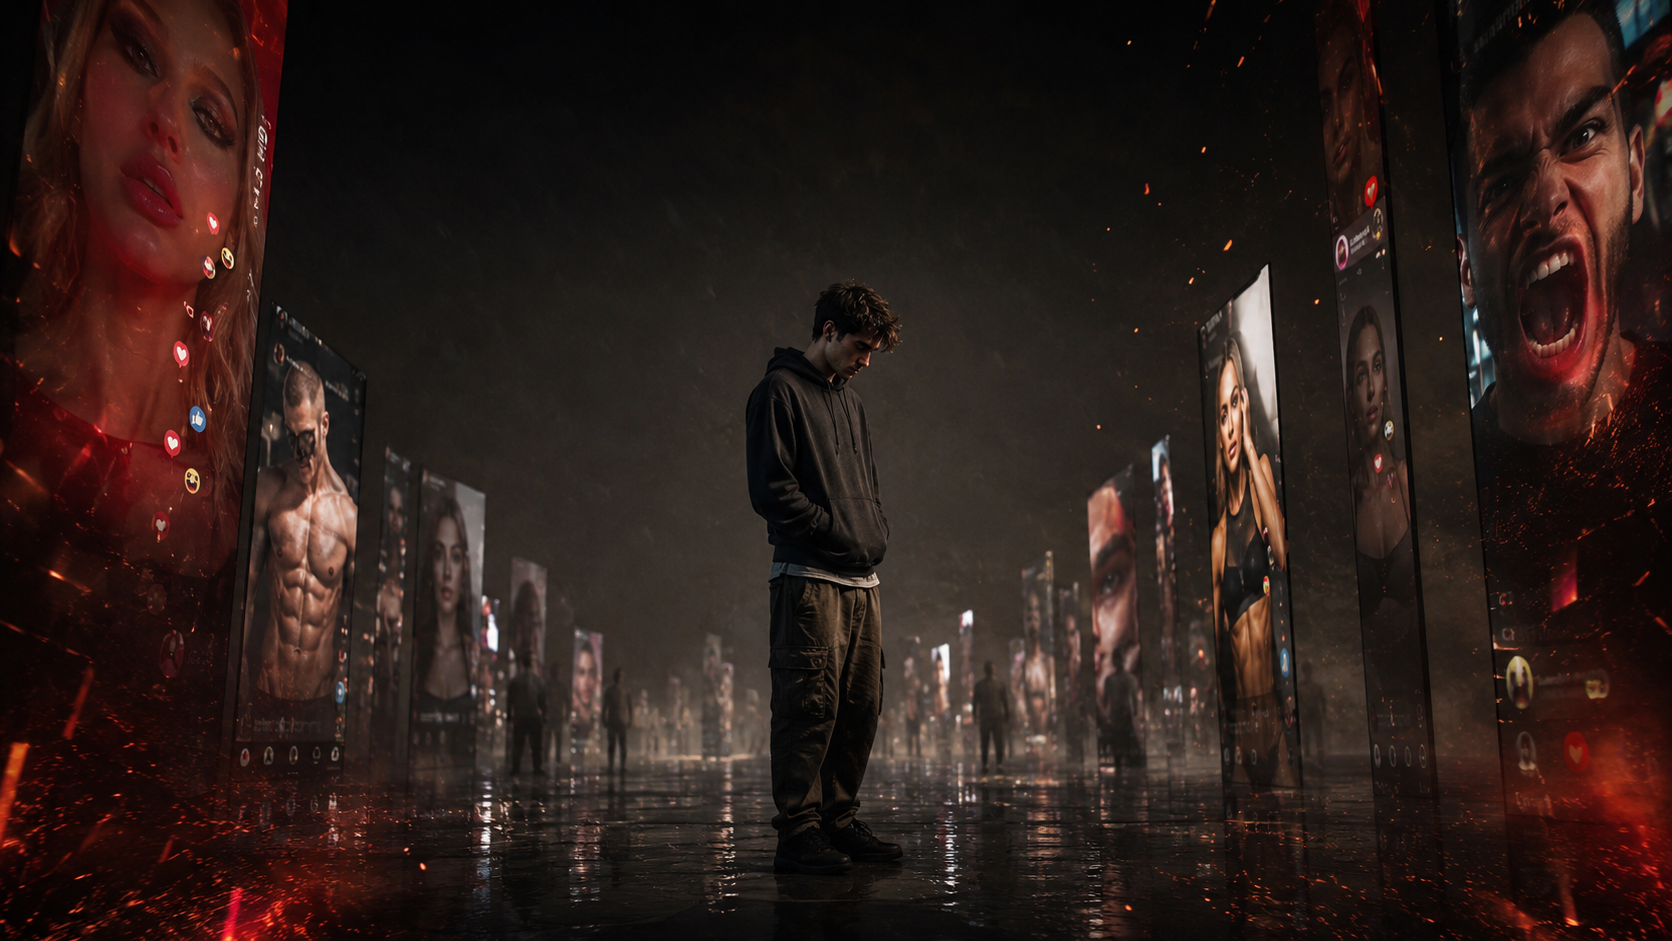
\includegraphics[keepaspectratio,alt={Chapter 02 cover}]{../assets/generated/covers/02_raised-by-the-algorithm_cover.png}}
\caption{Chapter 02 cover}
\end{figure}

\subsection{Opening}\label{opening}

We thought we were posting.

We were confessing.

We thought we were performing.

We were being measured.

We thought the feed was showing us the world.

The feed was teaching us which versions of ourselves would survive
inside it.

That last part matters because the deepest damage of the social era was
never just ``too much screen time.'' That phrase is way too soft. It
sounds like a lifestyle imbalance. What happened was closer to social
programming through ranked exposure. Not total programming. Not mind
control. Something more ordinary and therefore more powerful: repeated
incentives shaping what feels desirable, embarrassing, lovable,
aspirational, punishable, and real.

\subsection{Main Narrative}\label{main-narrative}

The algorithm did not invent insecurity. It industrialized it.

It did not invent vanity. It scaled it.

It did not invent loneliness. It learned how to monetize the gestures
people make when they are lonely.

This chapter is the emotional center of the first half of the book
because it gets closest to what readers already know in their bodies.
Brain fog. Comparison fatigue. Pornified aesthetics. Performance
pressure. Main-character exhaustion. The weird feeling that even private
life started sounding like content strategy. The sense that your
attention got cooked years before anyone around you had language for
what was happening.

That doesn't mean every wound in a generation can be pinned on social
media alone. That would be lazy and inaccurate. Economic precarity
matters. Housing pressure matters. Family instability matters. School
systems matter. The pandemic matters. Labor anxiety matters. But the
platform layer acted like an amplifier for all of it. It made insecurity
ambient, portable, and endlessly replayable.

That is the structural point.

The algorithm did not need to create every human weakness.

It only had to discover which arrangements of weakness kept people
watching.

\begin{figure}
\centering
\pandocbounded{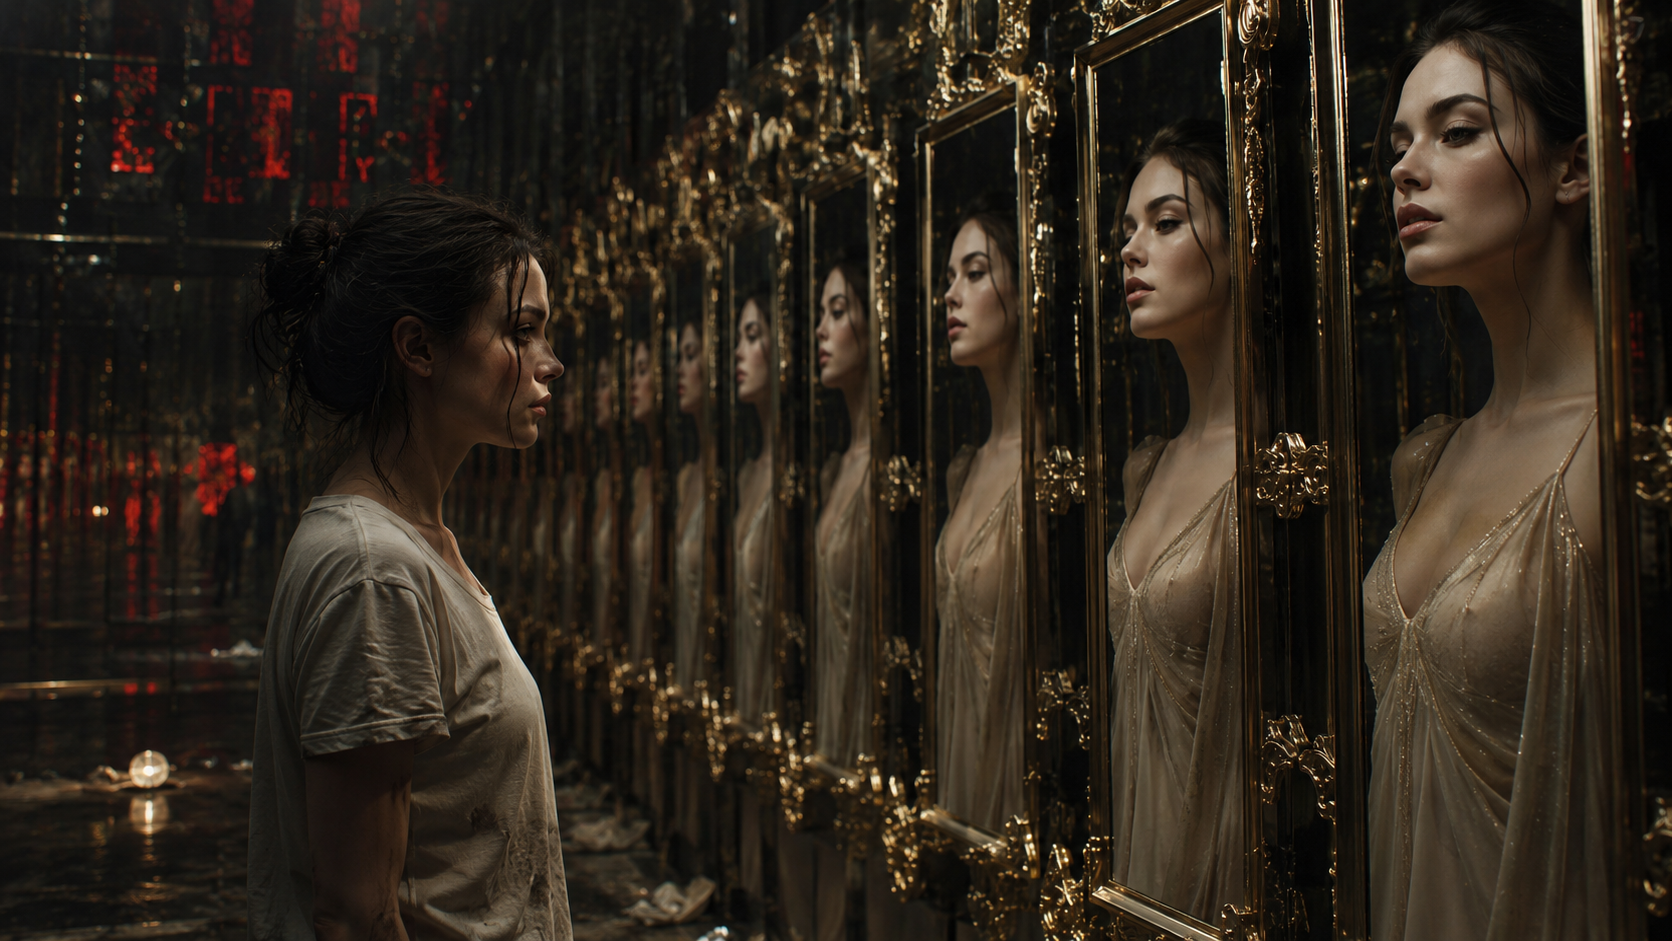
\includegraphics[keepaspectratio,alt={Chapter 02 narrative illustration A}]{../assets/generated/illustrations/02_raised-by-the-algorithm_scene_a.png}}
\caption{Chapter 02 narrative illustration A}
\end{figure}

That is why the cultural symptoms feel so familiar and so hard to
summarize at the same time. Hypersexualization becomes ordinary not
because desire is new, but because desire stripped into high-velocity
attention bait performs extremely well in ranking systems. Gangster
aesthetics become sticky not because violence is glamorous in some
eternal abstract sense, but because dominance, danger, and spectacle are
easy to package as scroll-stopping identity. Digital prostitution
aesthetics get normalized not because an entire generation woke up with
one shared moral collapse, but because the feed rewards monetized
intimacy and teaches users that visibility itself is survival.

The point here is not prudishness.

The point is incentive design.

\begin{figure}
\centering
\pandocbounded{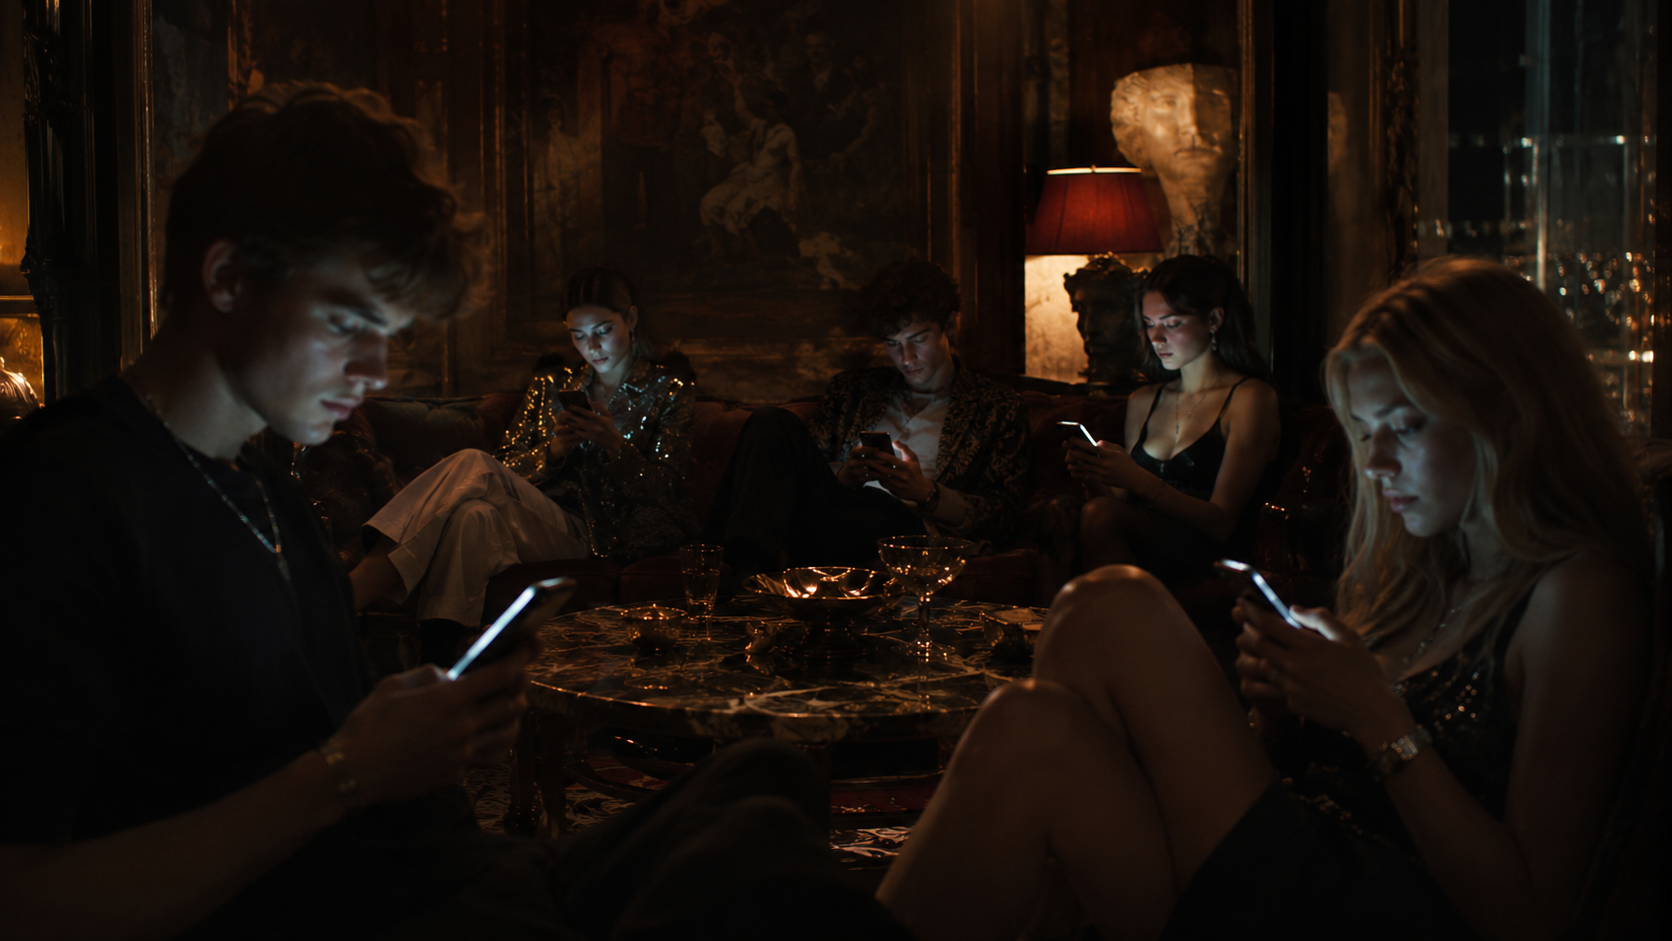
\includegraphics[keepaspectratio,alt={Chapter 02 narrative illustration}]{../assets/generated/illustrations/02_raised-by-the-algorithm_scene_c.png}}
\caption{Chapter 02 narrative illustration}
\end{figure}

The feed is not a neutral mirror reflecting culture back to itself. It
is an active ranking machine. It learns which emotions, fantasies,
humiliations, and social performances produce retention. Then it keeps
handing society more of what holds attention, even when what holds
attention also corrodes trust, stillness, self-respect, and judgment.

That is how a moral environment changes without anyone officially voting
to change it.

\begin{figure}
\centering
\pandocbounded{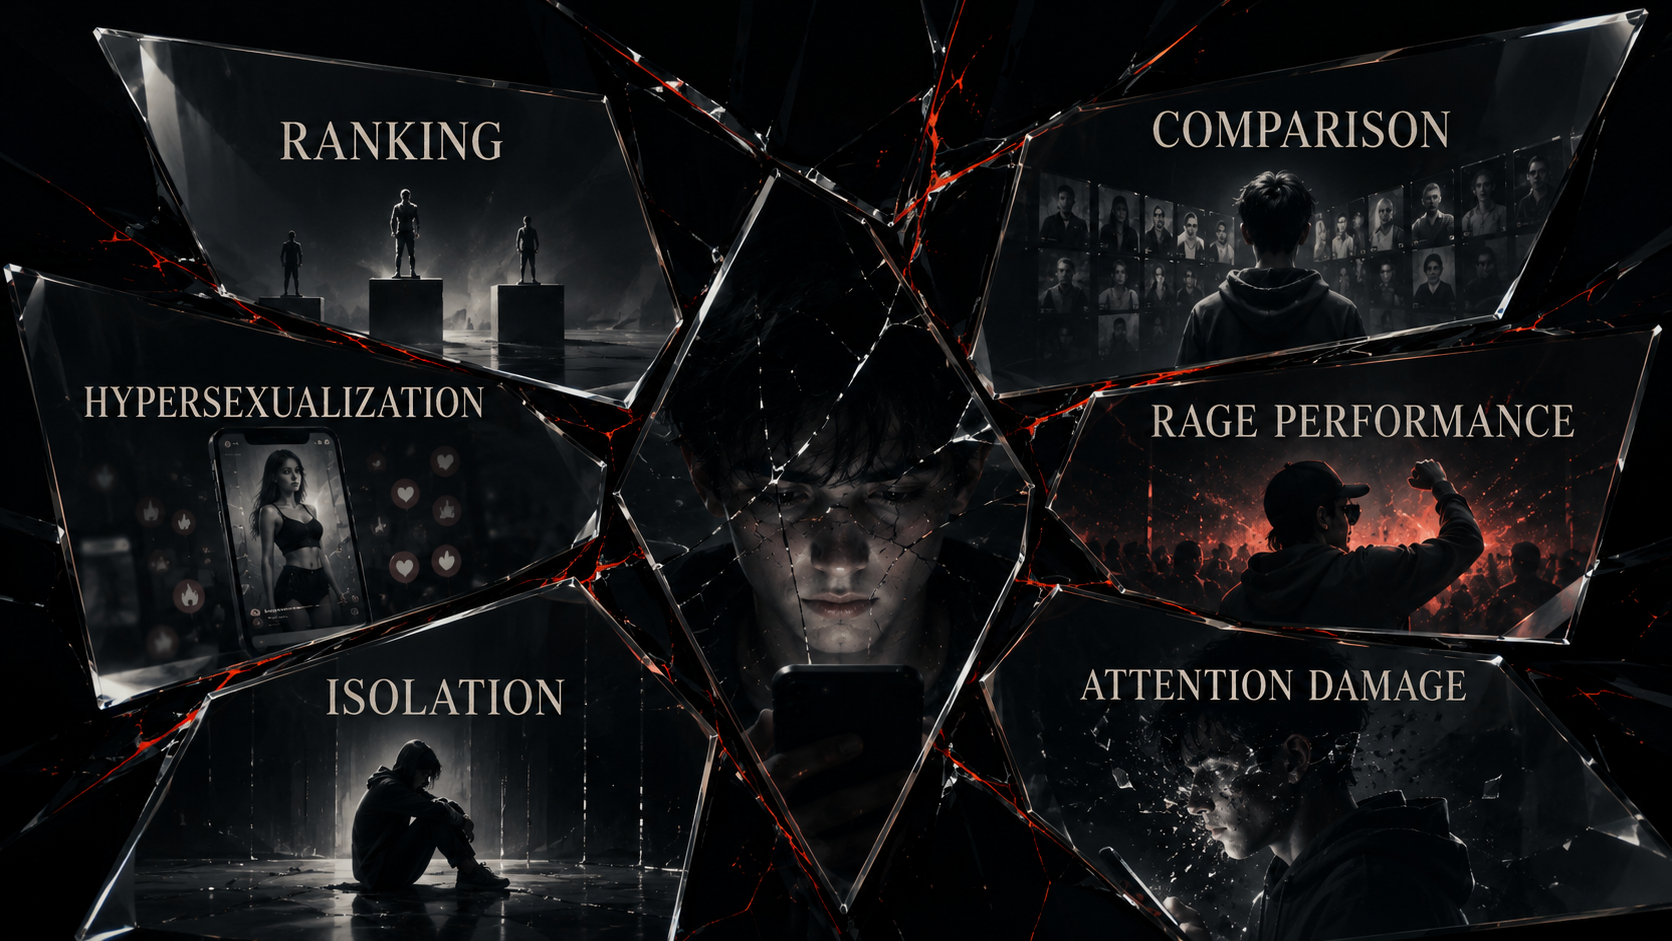
\includegraphics[keepaspectratio,alt={Chapter 02 infographic}]{../assets/generated/infographics/02_raised-by-the-algorithm_infographic_a.png}}
\caption{Chapter 02 infographic}
\end{figure}

This is also where the chapter has to be careful without going soft.
When this book talks about hypersexualization, prostitution aesthetics,
or gangster fantasy, it is not doing suburban pearl-clutching. It is
describing what happens when a ranking environment learns that certain
performances of body, power, danger, and humiliation convert beautifully
into attention. The algorithm did not force one single culture on
everyone. It rewarded the most extractable versions of culture. And over
time, the rewarded version starts looking like the normal version,
especially to kids whose social imagination was built inside the
machine.

That is why so many young people learned an awful lesson early: if you
want reach, flatten yourself into a stronger signal. Be hotter. Be
meaner. Be more available. Be more shameless. Be more watchable. Be more
broken in a way the app can aestheticize. Even authenticity starts
mutating under those conditions. The confession is no longer only a
confession. It is content pressure wearing the face of vulnerability.
The cry for connection gets mixed with performance because the system
keeps blurring the line between being seen and being fed into the next
ranking cycle.

A lot of people can feel this but still don't have a stable sentence for
it. They remember the before-and-after, even if the before is blurry
now. Before, some things still lived in distinct rooms: friendship,
embarrassment, flirting, gossip, aspiration, erotic life, boredom, play.
After enough years in the feed, those rooms began to collapse into one
another. Friendship became performance. Flirting became metrics.
Embarrassment became content. Boredom became danger because boredom
meant silence, and silence meant the feed might stop reflecting you
back.

That is one reason the psychological cost is so hard to explain to older
frameworks. A lot of adults still want to talk about ``bad influences''
as if the problem were mainly a set of wrong examples floating through
media. The platform era is more invasive than that. It changes the rate
at which identity is processed. It turns social life into constant
audience awareness. It makes ranking feel atmospheric. It trains people
to anticipate visibility the way earlier generations anticipated
weather.

And once that happens, the self gets tired in a new way.

Not just emotionally tired.

Context-switching tired.

Comparison tired.

Perform-or-vanish tired.

Always-legible tired.

That is why attention collapse belongs in this chapter as more than a
medical symptom. Yes, clinicians can and should talk about anxiety,
depression, compulsive use, and dysregulation in their own terms. But
this book is making an additional claim: mental-health decline is also
an infrastructure story. If a society places its youngest generations
inside systems engineered to interrupt stillness, weaponize comparison,
and reward arousal over reflection, then some portion of the resulting
distress is not a mysterious generational flaw. It is an operational
cost of the architecture.

That is a brutal sentence, but it is also clarifying.

Because generations that are constantly told they are fragile, lazy,
addicted, narcissistic, unserious, oversexualized, depoliticized,
hyperanxious, and unable to focus end up carrying a double burden. They
live inside the damage and then get blamed for not transcending it
individually.

The book rejects that move.

The claim here is not that young people are saints ruined by screens.

The claim is that vulnerability was systematized.

Fragility was industrialized.

Loneliness was monetized.

Status panic was optimized.

And then the generation most shaped by that process was mocked for
looking shaped.

This also helps explain why so many people feel ashamed of their own
habits while still returning to the systems that produce them.
Dependency in a technofeudal system is not just habit. It is social
necessity braided to emotional reward and punishment. Leaving the
platform or reducing dependence can feel like self-respect, but it can
also feel like disappearance. That tension is one reason shame becomes
such a powerful internal manager of behavior.

You know the app is bad for you.

You go back anyway.

You hate that you go back.

The shame makes you want stimulation.

The stimulation lives in the same app.

Now the loop manages itself.

That is not moral weakness in the shallow sense. It is behavioral design
meeting ordinary human vulnerability.

\begin{figure}
\centering
\pandocbounded{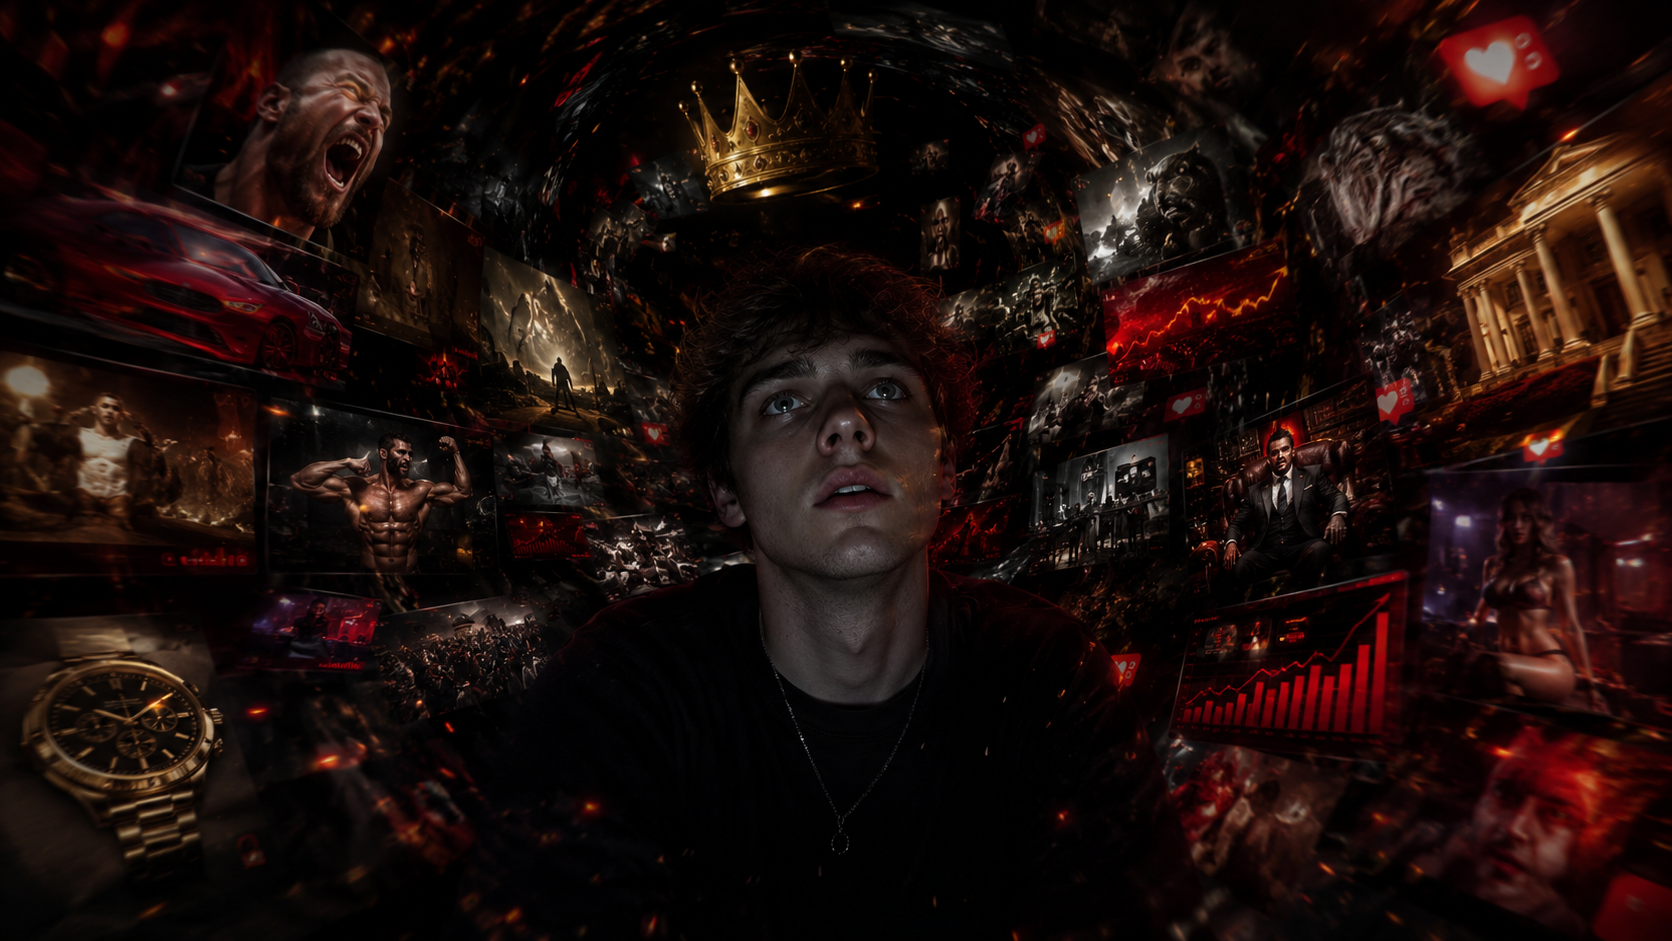
\includegraphics[keepaspectratio,alt={Chapter 02 narrative illustration B}]{../assets/generated/illustrations/02_raised-by-the-algorithm_scene_b.png}}
\caption{Chapter 02 narrative illustration B}
\end{figure}

And the violence is not only psychological. It is temporal. It steals
incubation. It steals the long awkward stretch in which a self used to
form a little more privately. Previous generations still had mirrors,
peer pressure, porn, status games, and cruelty. None of that began with
the phone. What changed is that the pressure became ambient, searchable,
replayable, and portable into the bed, the bathroom, the lunch table,
the walk home, the classroom, the family trip, the funeral, the
sleepless night. There is almost no private weather left in a life fully
raised by the feed.

The chapter also needs to say something careful about youth because the
differences between millennials and Gen Z matter. Millennials remember a
before. Not a pure before, not a perfect before, but a before in which
digital life had not yet swallowed everything. Gen Z, especially younger
Gen Z, was raised much more directly inside the platform-conditioned
world. For many, the feed was not an adoption story. It was childhood
weather. Their adolescence happened in public/private systems that
already knew how to rank faces, bodies, affiliations, jokes, aesthetics,
and emotional signals.

That is a profound developmental difference.

The child in a technofeudal order is not merely a future consumer.

The child is a native subject of the territory.

This is why the reforms at the end of the book have to reach beyond
moderation discourse. ``Better content policy'' does not begin to meet
the scale of what is being described here. The problem is not just a bad
post. It is a ranking environment that shapes the conditions under which
identity formation happens. Once you understand that, legal passivity
starts looking ridiculous. A platform that governs exposure, arousal,
and adolescent social reality at mass scale cannot keep hiding behind
the fiction that it merely hosts whatever people happen to upload.

It builds the social weather.

And the weather has consequences.

\subsection{Research Basis}\label{research-basis}

This chapter adapts the documentary argument developed in the research
paper
\href{../../papers/html/02_social-erosion-and-moral-reconfiguration_paper.html}{\textbf{Chapter
02: Social Erosion and Moral Reconfiguration}}. The PDF version is
\href{../../papers/pdf/02_social-erosion-and-moral-reconfiguration_paper/02_social-erosion-and-moral-reconfiguration_paper.pdf}{here}.
That paper ties youth harm, recommendation amplification, attention
damage, and moral reconfiguration back to platform design rather than to
simplistic civilizational decline stories.

\subsection{Next}\label{next}

Then history hit the accelerator. When the world shut down and life
moved even deeper into the screen, the platforms did not have to invent
a new dependence. They inherited a much larger one.

\end{document}
